% Written by paper/figures/src/v6_gallery.py; edit the script, not this file.
\begin{figure}[p]
  \centering
  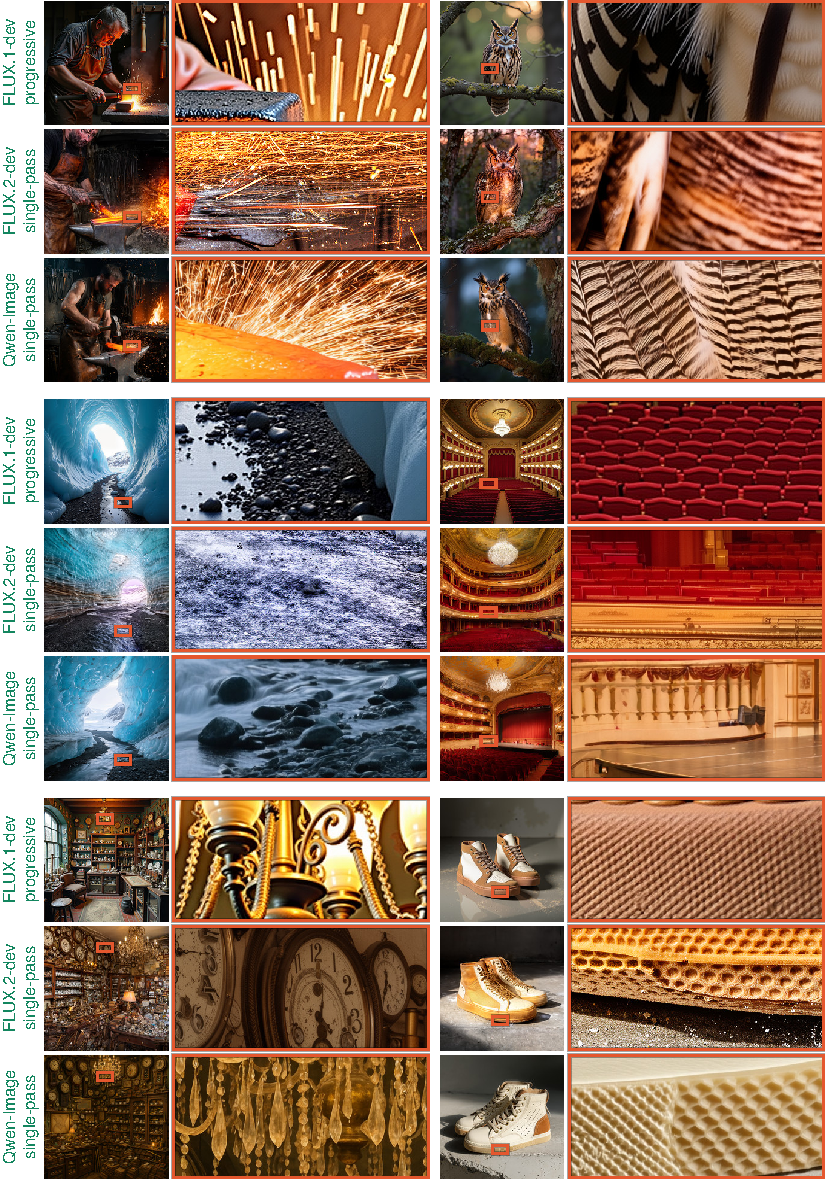
\includegraphics{figures/v6/showcase_models.pdf}
  \caption{\textbf{\sca{} carries native detail to FLUX.2-dev and Qwen-Image.} $4096^2$; progressive \sca{} on FLUX.1-dev (as in Figure~\ref{fig:prog_hero}) and single-pass \sca{} on FLUX.2-dev and Qwen-Image; one showcase prompt per category drawn with seed 0, seed 0 for every image. Each crop shows native pixels of the window that maximises the smallest edge energy among the three models.}
  \label{fig:showcase_models}
\end{figure}
